\section{测度的分解}
\label{sec:measure-decomposition}

第~\ref{sec:measure-relations}节的两种关系是两个极端：$\nu\ll\mu$时，$\nu$完全不在$\mu$的零测集上放质量；$\nu\perp\mu$时，$\nu$的全部质量都放在某个$\mu$零测集上。一般的测度介于两者之间，例如长度加上一个点质量。本节先证明：相对于给定的参考测度，任何$\sigma$有限测度都能唯一地拆成这两种极端之和；再在实轴上以Lebesgue测度为参考，把奇异部分进一步拆成点质量与“没有点质量的奇异质量”，并用Cantor集具体构造后者。整节只使用测度，不要求绝对连续部分能写成密度。

\subsection{Lebesgue分解}
\label{sec:measure-lebesgue-decomposition}

\paragraph{分解的陈述}
给定参考测度$\mu$与目标测度$\nu$，我们希望把$\nu$的质量分成两份：一份完全落在某个$\mu$零测集上，另一份在$\mu$零测集上没有任何质量。前者是$\mu$“看不见”的质量，后者是$\mu$能够“看见”的质量。

\begin{theorem}[Lebesgue分解]
\label{thm:measure-lebesgue-decomposition}
设$\mu$是可测空间$(X,\mathcal A)$上的非负测度，$\nu$是同一空间上的$\sigma$有限非负测度。则存在唯一的一对非负测度$\nu_{\mathrm{ac}},\nu_{\mathrm{s}}$，使
\[
 \nu=\nu_{\mathrm{ac}}+\nu_{\mathrm{s}},\qquad \nu_{\mathrm{ac}}\ll\mu,\qquad \nu_{\mathrm{s}}\perp\mu .
\]
这称为$\nu$相对于$\mu$的\term{Lebesgue分解}（Lebesgue decomposition），$\nu_{\mathrm{ac}}$与$\nu_{\mathrm{s}}$分别称为绝对连续部分与奇异部分。更具体地，存在$N\in\mathcal A$使$\mu(N)=0$，并且$\nu_{\mathrm{s}}(A)=\nu(A\cap N)$，$\nu_{\mathrm{ac}}(A)=\nu(A\setminus N)$。
\end{theorem}

分解总是相对于参考测度的。在实轴上取$\nu=\lambda|_{[0,1]}+\delta_2$。以$\lambda$为参考时，$N=\{2\}$是$\lambda$零测集且承载点质量，于是$\nu_{\mathrm{s}}=\delta_2$，$\nu_{\mathrm{ac}}=\lambda|_{[0,1]}$。以$\delta_2$为参考时，$\delta_2$的零测集是不含点$2$的集合，取$N=\mathbb R\setminus\{2\}$，于是角色互换：$\nu_{\mathrm{s}}=\lambda|_{[0,1]}$，$\nu_{\mathrm{ac}}=\delta_2$。同一个$\nu$换一个参考，同一份质量就可能从一个部分换到另一个部分，见图~\ref{fig:measure-lebesgue-decomposition}。

\begin{figure}[!htbp]
  \centering
  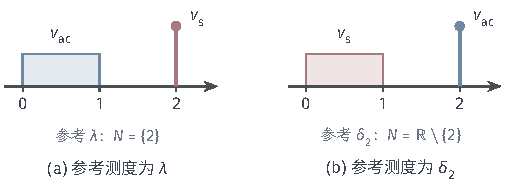
\includegraphics[width=85.672mm]{figures/02-abstract-mathematics/01-metric-and-measure/tikz/c2-lebesgue-decomposition/figure.pdf}
  \caption{Lebesgue分解依赖参考测度。$\nu=\lambda|_{[0,1]}+\delta_2$，蓝色为绝对连续部分，红色为奇异部分。(a)以$\lambda$为参考，点$2$是$\lambda$零测集，点质量是奇异部分；(b)以$\delta_2$为参考，$\mathbb R\setminus\{2\}$是$\delta_2$零测集，区间上的长度变成奇异部分。}
  \label{fig:measure-lebesgue-decomposition}
\end{figure}

\paragraph{有限情形：选取承载最多质量的零测集}
定理中的集合$N$应当尽可能多地装下$\nu$的质量，同时保持$\mu(N)=0$。若某个$\mu$零测集在$N$之外还有正的$\nu$质量，就把它并进$N$。这个“装到不能再装”的想法可以用上确界实现。我们先在$\nu$有限时证明存在性。

\begin{proof}[定理~\ref{thm:measure-lebesgue-decomposition}在$\nu$有限时的存在性]
令
\[
 M=\sup\{\nu(A):A\in\mathcal A,\ \mu(A)=0\}.
\]
空集在集合族中，所以$M\ge0$；又$M\le\nu(X)<\infty$。对每个$k$取$\mu$零测集$N_k$使$\nu(N_k)>M-1/k$，并令$N=\bigcup_kN_k$。由可数次可加性，$\mu(N)\le\sum_k\mu(N_k)=0$，所以$N$本身也在集合族中，$\nu(N)\le M$；另一方面$\nu(N)\ge\nu(N_k)>M-1/k$对每个$k$成立，故$\nu(N)=M$。上确界被$N$达到。

令$\nu_{\mathrm{s}}(A)=\nu(A\cap N)$，$\nu_{\mathrm{ac}}(A)=\nu(A\setminus N)$。两者都是$\nu$限制到可测子集所得的测度，且$\nu=\nu_{\mathrm{ac}}+\nu_{\mathrm{s}}$。由$\mu(N)=0$与$\nu_{\mathrm{s}}(X\setminus N)=0$得$\nu_{\mathrm{s}}\perp\mu$。

剩下证明$\nu_{\mathrm{ac}}\ll\mu$。设$\mu(A)=0$，则$N\cup(A\setminus N)$仍是$\mu$零测集，其$\nu$质量不超过$M$。这两部分不交，所以
\[
 M+\nu(A\setminus N)=\nu(N)+\nu(A\setminus N)\le M .
\]
$M$有限，可以从两边消去，得$\nu_{\mathrm{ac}}(A)=\nu(A\setminus N)=0$。
\end{proof}

最后一步的“消去”正是需要$\nu$有限的地方：若$M=+\infty$，不等式$M+t\le M$不能推出$t=0$。

\paragraph{$\sigma$有限情形与唯一性}
$\sigma$有限测度可以切成可数个有限片，在每片上重复上面的构造，再把各片的零测集合并。

\begin{proof}[定理~\ref{thm:measure-lebesgue-decomposition}在一般情形下的存在性与唯一性]
\emph{存在性。}由$\sigma$有限性，取两两不交的$X_1,X_2,\dots\in\mathcal A$使$\bigcup_jX_j=X$且$\nu(X_j)<\infty$。对每个$j$，有限测度$\nu_j(A)=\nu(A\cap X_j)$满足已证情形，得到$\mu$零测集$N_j'$；用$N_j=N_j'\cap X_j$代替它，仍有$\mu(N_j)=0$，且$\nu_j(A\setminus N_j)=\nu_j(A\setminus N_j')$对所有$A$成立，因为$\nu_j$在$X_j$之外没有质量。令$N=\bigcup_jN_j$，则$\mu(N)=0$。定义$\nu_{\mathrm{s}}(A)=\nu(A\cap N)$，$\nu_{\mathrm{ac}}(A)=\nu(A\setminus N)$，同前有$\nu_{\mathrm{s}}\perp\mu$。若$\mu(A)=0$，由$N\cap X_j=N_j$，
\[
 \nu_{\mathrm{ac}}(A)=\sum_j\nu\bigl((A\setminus N)\cap X_j\bigr)=\sum_j\nu_j(A\setminus N_j)=0,
\]
最后一步是各片上已证的绝对连续性。

\emph{唯一性。}设$\nu=\alpha+\beta=\alpha'+\beta'$，其中$\alpha,\alpha'\ll\mu$，$\beta,\beta'\perp\mu$。取$\mu$零测集$S,S'$使$\beta(X\setminus S)=0$，$\beta'(X\setminus S')=0$，令$T=S\cup S'$，则$\mu(T)=0$，且$\beta,\beta'$在$X\setminus T$上都没有质量。对任意$A\in\mathcal A$，$\mu(A\cap T)=0$推出$\alpha(A\cap T)=\alpha'(A\cap T)=0$，因此
\[
 \beta(A\cap T)=\nu(A\cap T)=\beta'(A\cap T);
\]
又$\beta(A\setminus T)=\beta'(A\setminus T)=0$，因此$\alpha(A\setminus T)=\nu(A\setminus T)=\alpha'(A\setminus T)$。把$A\cap T$与$A\setminus T$上的值相加，得$\alpha=\alpha'$，$\beta=\beta'$。
\end{proof}

唯一性的论证只在两个集合上分别读取$\nu$，没有做减法。整个证明用到的只是可数次可加性、上确界与限制测度，没有用到积分、Hahn分解或任何密度。

存在性中的$\sigma$有限条件不能随意去掉。在$[0,1]$的Borel可测空间上取$\mu=\lambda$，$\nu$为计数测度，它不是$\sigma$有限的（可数个有限测度集都是有限集，并起来只是可数集）。若$\nu=\nu_{\mathrm{ac}}+\nu_{\mathrm{s}}$满足定理的要求，取$N$使$\lambda(N)=0$、$\nu_{\mathrm{s}}([0,1]\setminus N)=0$。由于$\lambda(N)=0$，$N\ne[0,1]$，取$x\notin N$，则$\nu_{\mathrm{s}}(\{x\})=0$，而$\lambda(\{x\})=0$又给出$\nu_{\mathrm{ac}}(\{x\})=0$，于是$\nu(\{x\})=0$，与计数测度给单点质量$1$矛盾。

第~\ref{chap:densities-change-of-measure}章将回答下一个问题：绝对连续部分$\nu_{\mathrm{ac}}$在什么条件下能写成参考测度$\mu$的加权形式。那是在积分建立之后，对已经分出的绝对连续质量寻找函数表示；本节的分解并不依赖它。

\subsection{实轴上的三元分解}
\label{sec:measure-three-part}

在实轴上以Lebesgue测度为参考时，奇异部分还可以再分。单点都是$\lambda$零测集，所以点质量一定属于奇异部分；问题是奇异部分是否只有点质量。下面先把点质量完整地提出来，再说明余下的奇异部分可以不为零。

\paragraph{点质量至多可数}
设$\rho$是$\mathcal B(\mathbb R)$上的有限测度。若$\rho(\{x\})>0$，称$x$是$\rho$的一个原子，即带正质量的单点。

\begin{lemma}[正质量单点至多可数]
\label{lem:measure-atoms-countable}
有限Borel测度$\rho$的原子集$A=\{x\in\mathbb R:\rho(\{x\})>0\}$至多可数。
\end{lemma}

\begin{proof}
按质量的正下界分组：令$A_k=\{x:\rho(\{x\})>1/k\}$，则$A=\bigcup_kA_k$。若$x_1,\dots,x_m$是$A_k$中互不相同的点，有限可加性与单调性给出$m/k<\sum_{i=1}^m\rho(\{x_i\})\le\rho(\mathbb R)$，所以$A_k$至多有$k\rho(\mathbb R)$个点。可数个有限集之并至多可数。
\end{proof}

于是可以定义$\rho_{\mathrm d}(B)=\rho(B\cap A)$。由于$A$至多可数，可数可加性给出
\[
 \rho_{\mathrm d}(B)=\sum_{x\in A\cap B}\rho(\{x\}),
\]
它是全部点质量之和，称为$\rho$的离散部分。余下的$\rho_{\mathrm c}(B)=\rho(B\setminus A)$没有原子：$x\in A$时$\rho_{\mathrm c}(\{x\})=0$，$x\notin A$时$\rho_{\mathrm c}(\{x\})=\rho(\{x\})=0$。

\begin{theorem}[实轴上有限测度的三元分解]
\label{thm:measure-three-part}
设$\rho$是$\mathcal B(\mathbb R)$上的有限测度。则$\rho$可以唯一地写成
\[
 \rho=\rho_{\mathrm d}+\rho_{\mathrm{ac}}+\rho_{\mathrm{sc}},
\]
其中$\rho_{\mathrm d}$集中在一个至多可数集上，$\rho_{\mathrm{ac}}\ll\lambda$，$\rho_{\mathrm{sc}}\perp\lambda$且$\rho_{\mathrm{sc}}$没有原子。没有原子且与$\lambda$相互奇异的测度称为\term{奇异连续测度}（singular continuous measure）。
\end{theorem}

\begin{proof}
存在性：$\rho_{\mathrm d}$与$\rho_{\mathrm c}$如上定义。对有限测度$\rho_{\mathrm c}$关于$\lambda$作Lebesgue分解，得$\rho_{\mathrm c}=\rho_{\mathrm{ac}}+\rho_{\mathrm{sc}}$。$\rho_{\mathrm{sc}}(\{x\})\le\rho_{\mathrm c}(\{x\})=0$，所以$\rho_{\mathrm{sc}}$没有原子。

唯一性：设$\rho=d+a+s$也满足条件，$d$集中在至多可数集$D$上。$a\ll\lambda$与$\lambda(\{x\})=0$给出$a(\{x\})=0$，而$s$没有原子，所以$\rho(\{x\})=d(\{x\})$对每个$x$成立。于是
\[
 d(B)=\sum_{x\in B\cap D}d(\{x\})=\sum_{x\in B\cap D}\rho(\{x\})=\sum_{x\in B\cap A}\rho(\{x\})=\rho_{\mathrm d}(B),
\]
第一个等号用了$d$集中在可数集$D$上及可数可加性。第三个等号成立，是因为$D$中质量为零的点不贡献，而$A\subseteq D$：若$\rho(\{x\})>0$，则$d(\{x\})=\rho(\{x\})>0$，而$d$在$D$之外没有质量，故$x\in D$。由此$a+s=\rho-d=\rho_{\mathrm c}$（各项有限，减法有意义），再由定理~\ref{thm:measure-lebesgue-decomposition}的唯一性得$a=\rho_{\mathrm{ac}}$，$s=\rho_{\mathrm{sc}}$。
\end{proof}

离散部分集中在可数集$A$上，而$\lambda(A)=0$，所以$\rho_{\mathrm d}\perp\lambda$；$\rho$相对于$\lambda$的Lebesgue奇异部分就是$\rho_{\mathrm d}+\rho_{\mathrm{sc}}$。三项是\emph{同一个测度的三个成分}，一个测度可以同时含有三者，也可以缺少其中任意几项；它们不是把测度分成三个互斥类别。

三项中的离散部分可以从累计函数读出。记$G(x)=\rho((-\infty,x])$。集合$(-\infty,x-1/m]$递增到$(-\infty,x)$，由测度从下连续性，$G(x-)=\rho((-\infty,x))$，所以
\[
 G(x)-G(x-)=\rho(\{x\}),
\]
这与第~\ref{sec:measure-construction}节中Lebesgue–Stieltjes测度的单点质量公式一致。因此$G$在$x$处跳跃当且仅当$x$是原子，$G$连续当且仅当$\rho_{\mathrm d}=0$。累计函数连续能排除离散部分，却不能排除奇异连续部分；下面的例子说明后者确实存在。

\paragraph{Cantor函数}
回到第~\ref{sec:measure-construction}节构造的Cantor集$C=\bigcap_nC_n$（图~\ref{fig:measure-cantor-set}），其中$C_n$由$2^n$个长度为$3^{-n}$的闭区间组成，$\lambda(C_n)=(2/3)^n$，$\lambda(C)=0$。我们要构造一个连续的单调函数，它只在$C$上增长：每一步把增量平均分给保留下来的区间，删去的开区间上不再增长。

令$F_0(x)=x$（$0\le x\le1$）。设$F_n$已经定义：它在$[0,1]$上连续、单调不减，$F_n(0)=0$，$F_n(1)=1$，在$C_n$的每个区间上线性增长$2^{-n}$，在已删去的开区间上为常数。构造$F_{n+1}$时，只在$C_n$的每个区间$J=[a,a+3^{-n}]$上修改：$J$被三等分，$F_{n+1}$在左右两段上各线性增长$2^{-n-1}$，在中间开区间上取常数$F_n(a)+2^{-n-1}$；在$J$之外令$F_{n+1}=F_n$。$F_{n+1}$在$J$的两端与$F_n$取值相同，所以修改后仍连续、单调，且满足同样的描述。

在区间$J$内，$F_{n+1}-F_n$在左三分之一上从$0$线性增大到$2^{-n}(\tfrac12-\tfrac13)=2^{-n}/6$，在中间三分之一上线性减小到$-2^{-n}/6$，在右三分之一上回到$0$，所以
\[
 \sup_{x\in[0,1]}|F_{n+1}(x)-F_n(x)|=\frac{2^{-n}}{6}.
\]
对$m>n$，逐项相加得$\sup_x|F_m(x)-F_n(x)|\le\sum_{j\ge n}2^{-j}/6=2^{-n}/3$。因此每个$x$处的数列$(F_n(x))$是Cauchy列，极限$F(x)=\lim_nF_n(x)$存在，并且$\sup_x|F(x)-F_n(x)|\le2^{-n}/3$：函数列一致收敛。

\begin{example}[在$x=1/4$处逐步计算]
$1/4$不在任何被删去的开区间中，它在每一步都落在某个保留区间内。逐步计算（$F_0(1/4)=1/4$）：
\[
 F_1\bigl(\tfrac14\bigr)=\tfrac38,\quad F_2\bigl(\tfrac14\bigr)=\tfrac5{16},\quad F_3\bigl(\tfrac14\bigr)=\tfrac{11}{32},\quad F_4\bigl(\tfrac14\bigr)=\tfrac{21}{64}.
\]
例如$F_2$在$[2/9,1/3]$上从$1/4$线性增长到$1/2$，而$1/4-2/9=1/36$是该区间长度$1/9$的四分之一，故$F_2(1/4)=1/4+\tfrac14\cdot\tfrac14=5/16$。相邻两项之差依次为$1/8,1/16,1/32,1/64$，都不超过上面的界$2^{-n}/6$，数列交替逼近$F(1/4)=1/3$。若读者熟悉进位制，可以这样核对极限：$1/4$的三进制展开为$0.020202\ldots$，把数字$2$换成$1$并按二进制读出$0.010101\ldots=1/3$。
\end{example}

\begin{figure}[!htbp]
  \centering
  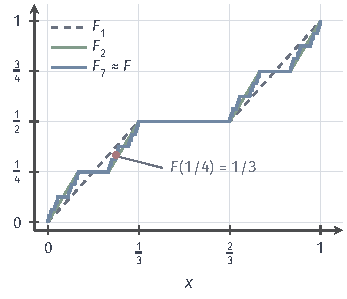
\includegraphics[width=58.815mm]{figures/02-abstract-mathematics/01-metric-and-measure/tikz/c2-cantor-function/figure.pdf}
  \caption{Cantor函数的逐步构造。虚线为$F_1$，绿色为$F_2$，蓝色为$F_7$，后者与极限$F$的一致误差不超过$2^{-7}/3$。每一步只在保留区间上增长，在删去的开区间上保持水平；红点为$F(1/4)=1/3$。}
  \label{fig:measure-cantor-function}
\end{figure}

极限函数$F$称为\term{Cantor函数}（Cantor function），图~\ref{fig:measure-cantor-function}画出了它的近似。它继承了以下性质。第一，$F$单调不减，$F(0)=0$，$F(1)=1$，因为每个$F_n$如此，不等式与等式在逐点极限下保持。第二，$F$连续：任给$\varepsilon>0$，取$n$使$2^{-n}/3<\varepsilon/3$，再由$F_n$连续取$\delta$使$|x-y|<\delta$时$|F_n(x)-F_n(y)|<\varepsilon/3$，则
\[
 |F(x)-F(y)|\le|F(x)-F_n(x)|+|F_n(x)-F_n(y)|+|F_n(y)-F(y)|<\varepsilon .
\]
第三，$F$在每个删去的开区间上为常数：第$k$步删去的开区间位于$C_k$之外，此后每一步都不再修改它上面的值。第四，在$C_n$的每个区间$[a,b]$上，$F(b)-F(a)=2^{-n}$，因为以后的修改都不改变区间端点的值。

\paragraph{Cantor测度}
把$F$延拓到整条实轴：$x<0$时$F(x)=0$，$x>1$时$F(x)=1$。延拓后的$F$连续、单调不减、取有限值，满足第~\ref{sec:measure-construction}节中Lebesgue–Stieltjes构造的条件，于是存在Borel测度$\mu_C$使$\mu_C((a,b])=F(b)-F(a)$。称$\mu_C$为\term{Cantor测度}（Cantor measure）。

它的三条性质都可以用前面的结论直接核对。总质量为$\mu_C(\mathbb R)=\lim_m(F(m)-F(-m))=1$。没有原子：$F$连续，所以$\mu_C(\{x\})=F(x)-F(x-)=0$。集中在$C$上：$\mathbb R\setminus C$是$(-\infty,0)$、$(1,\infty)$与可数个删去的开区间之并；在每个这样的开区间$(a,b)$上$F$为常数，由从下连续性，
\[
 \mu_C((a,b))=\lim_{m\to\infty}\mu_C\bigl((a,b-\tfrac1m]\bigr)=\lim_{m\to\infty}\bigl(F(b-\tfrac1m)-F(a)\bigr)=0,
\]
两条半直线同理；由可数次可加性，$\mu_C(\mathbb R\setminus C)=0$。又$\lambda(C)=0$，所以取$N=C$即得$\mu_C\perp\lambda$。

这样，$\mu_C$是一个非零的奇异连续测度：它的累计函数$F$处处连续，没有任何点质量，却把全部质量放在一个长度为零的集合上。由$F$的第四条性质，$\mu_C$给$C_n$的每个区间$[a,b]$的质量为$F(b)-F(a-)=F(b)-F(a)=2^{-n}$，所以$\mu_C(C_n)=2^n\cdot2^{-n}=1$；同一列集合的长度$(2/3)^n$却趋于零。图~\ref{fig:measure-cantor-mass-length}并排画出这两个数列：长度测度越来越看不见的集合，始终承载着Cantor测度的全部质量。

\begin{figure}[!htbp]
  \centering
  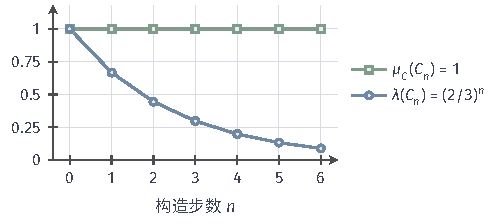
\includegraphics[width=84.691mm]{figures/02-abstract-mathematics/01-metric-and-measure/tikz/c2-cantor-mass-length/figure.pdf}
  \caption{同一列集合$C_n$在两种测度下的质量。蓝色圆点为长度$\lambda(C_n)=(2/3)^n$，$n=0,\dots,6$时从$1$降到约$0.088$；绿色方点为Cantor测度$\mu_C(C_n)=1$，保持不变。由从上连续性，两者的极限分别给出$\lambda(C)=0$与$\mu_C(C)=1$，所以$\mu_C\perp\lambda$。}
  \label{fig:measure-cantor-mass-length}
\end{figure}第~\ref{sec:integral-differentiation}节将再次使用Cantor函数，检验由导数恢复函数增量的公式何时失效。

\paragraph{三类成分的混合}
三种成分可以出现在同一个测度中。令
\[
 \rho=\tfrac12\lambda|_{[0,1]}+\tfrac14\delta_{1/2}+\tfrac14\mu_C .
\]
它是三个有限测度的非负加权和，总质量$\tfrac12+\tfrac14+\tfrac14=1$。累计函数在$[0,1]$上为
\[
 G(x)=\tfrac12x+\tfrac14\mathbf 1_{[1/2,\infty)}(x)+\tfrac14F(x).
\]
由于$1/2$位于删去的区间$(1/3,2/3)$中，$F(1/2)=1/2$，所以$G(1/2-)=\tfrac14+\tfrac18=\tfrac38$，$G(1/2)=\tfrac38+\tfrac14=\tfrac58$，跳跃$\tfrac14$恰是点$1/2$的质量；又如$G(1/4)=\tfrac18+\tfrac1{12}=\tfrac5{24}$。

按定理~\ref{thm:measure-three-part}的步骤分解：唯一的原子是$1/2$，因为$\lambda$与$\mu_C$都没有原子，故$\rho_{\mathrm d}=\tfrac14\delta_{1/2}$；余下的$\tfrac12\lambda|_{[0,1]}+\tfrac14\mu_C$相对于$\lambda$作Lebesgue分解，取$N=C$，前一项在$C$上为零、后一项集中在$C$上，得$\rho_{\mathrm{ac}}=\tfrac12\lambda|_{[0,1]}$，$\rho_{\mathrm{sc}}=\tfrac14\mu_C$。图~\ref{fig:measure-three-part-decomposition}对照了三个分量的累计函数与它们的和。从$G$的图像只能直接读出跳跃；连续增长的部分哪些来自长度、哪些来自Cantor测度，单看“连续”无法区分。第~\ref{chap:densities-change-of-measure}章将用Radon–Nikodym定理说明，绝对连续部分可以由相对于$\lambda$的密度表示，而奇异连续部分不能。

\begin{figure}[!htbp]
  \centering
  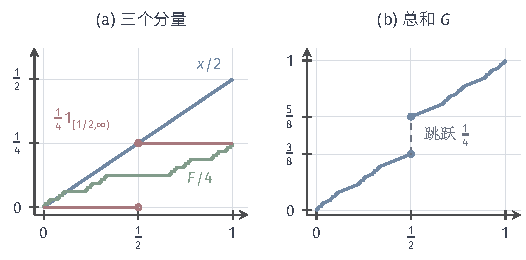
\includegraphics[width=88.999mm]{figures/02-abstract-mathematics/01-metric-and-measure/tikz/c2-three-part-decomposition/figure.pdf}
  \caption{实轴上三类成分的混合$\rho=\tfrac12\lambda|_{[0,1]}+\tfrac14\delta_{1/2}+\tfrac14\mu_C$。(a)三个分量的累计函数：蓝色直线$x/2$来自长度，红色阶跃来自点质量，绿色阶梯状曲线$F/4$来自Cantor测度（以$F_7$近似）。(b)总和$G$在$1/2$处从$3/8$跳到$5/8$，其余部分连续；跳跃对应离散部分，连续增长中既有绝对连续部分，也有奇异连续部分。}
  \label{fig:measure-three-part-decomposition}
\end{figure}
